\documentclass[12pt,a4paper]{article} 
\usepackage[latin1]{inputenc}
\usepackage{pdfpages}
\usepackage{graphicx}
\usepackage{float}
\usepackage{amsmath} 
\usepackage{amsfonts} 
\usepackage{amssymb}
\usepackage{color}
\usepackage{multicol}
\usepackage{multirow}
\usepackage{makeidx} 
\usepackage[english]{babel} 
\usepackage[hidelinks]{hyperref} 
\usepackage{array}
\usepackage{blindtext}
\usepackage{setspace}
\usepackage{parskip}

\usepackage{pstricks}
\linespread{1.1}
\begin{document}
\definecolor{PSU}{RGB}{75,125,50}
\begin{titlepage}
\begin{center}

% leave tilde after graphic, it designates par format, needed for formating

\includegraphics[width=.75\textwidth]{./PSU_logo.png}~\\[.5cm]

\textsc{\LARGE \color{PSU} Maseeh College of Engineering}\\[1.5cm]

\textsc{\Large Project Proposal}\\[0.5cm]
\textsc{\Large Submission Draft \#3.0}\\[0.5cm]
\vspace{1cm}
% Title

{ \huge \bfseries\color{PSU} A Block of Code\\[0.4cm] }
  \large Senior Capstone Project

% \hrule
\vspace{2.5cm}
% Team Members
 \begin{multicols}{2}

\begin{flushleft}
\noindent
 \large
\emph{\color{PSU}Team Members:}\\
Nathan \textsc{Bryant}\\
Daniel \textsc{Frister}\\
Tyler  \textsc{Hart}\\
Jacob   \textsc{Micikiewicz}\\
Greg    \textsc{Stromire}\\
\end{flushleft}

 \begin{flushleft}
  \large
 \emph{\color{PSU}Erebus Labs:} \\
 Dr. Mike  \textsc{Borowczak}\\
 \emph{\color{PSU}University of Wyoming}\\
 DR. Andrea \textsc{Burrows}\\
 \emph{\color{PSU}PSU Advisor:}\\
 Roy \textsc{Kravitz}
 \end{flushleft}


 \end{multicols}`
\vfill

% Bottom of the page
{\large \today}

\end{center}
\end{titlepage}
 \tableofcontents

\section{Needs Statement}
Today's world is one of interconnected technologies, at the heart of which are devices like computers and micro-controllers. As the technological complexity of our world increases we will find our society increasingly reliant on the men and women who know how to operate and control these devices.


However as of today no universally accessible curriculum includes a focus on the knowledge and skills needed to program these machines. We have need of any system that can help children learn and understand these concepts. Additionally,  the long term effectiveness of any system will depend on both it's ease of use and it's accessibility across a large range communities, especially those under financial duress.


\section{Objective}
The primary goal of this project is to create a low cost tactile teaching aide capable of helping a wide range  K-12 students learn the basics of computer programming. Our proposed teaching aide is a set of blocks that will allow students to  perform basic programming operations and assignments through the arrangement of the blocks. Verification of valid code structures will provide feedback for learning, and control of simple outputs connected to the system can give students a goal for their projects.
\newpage

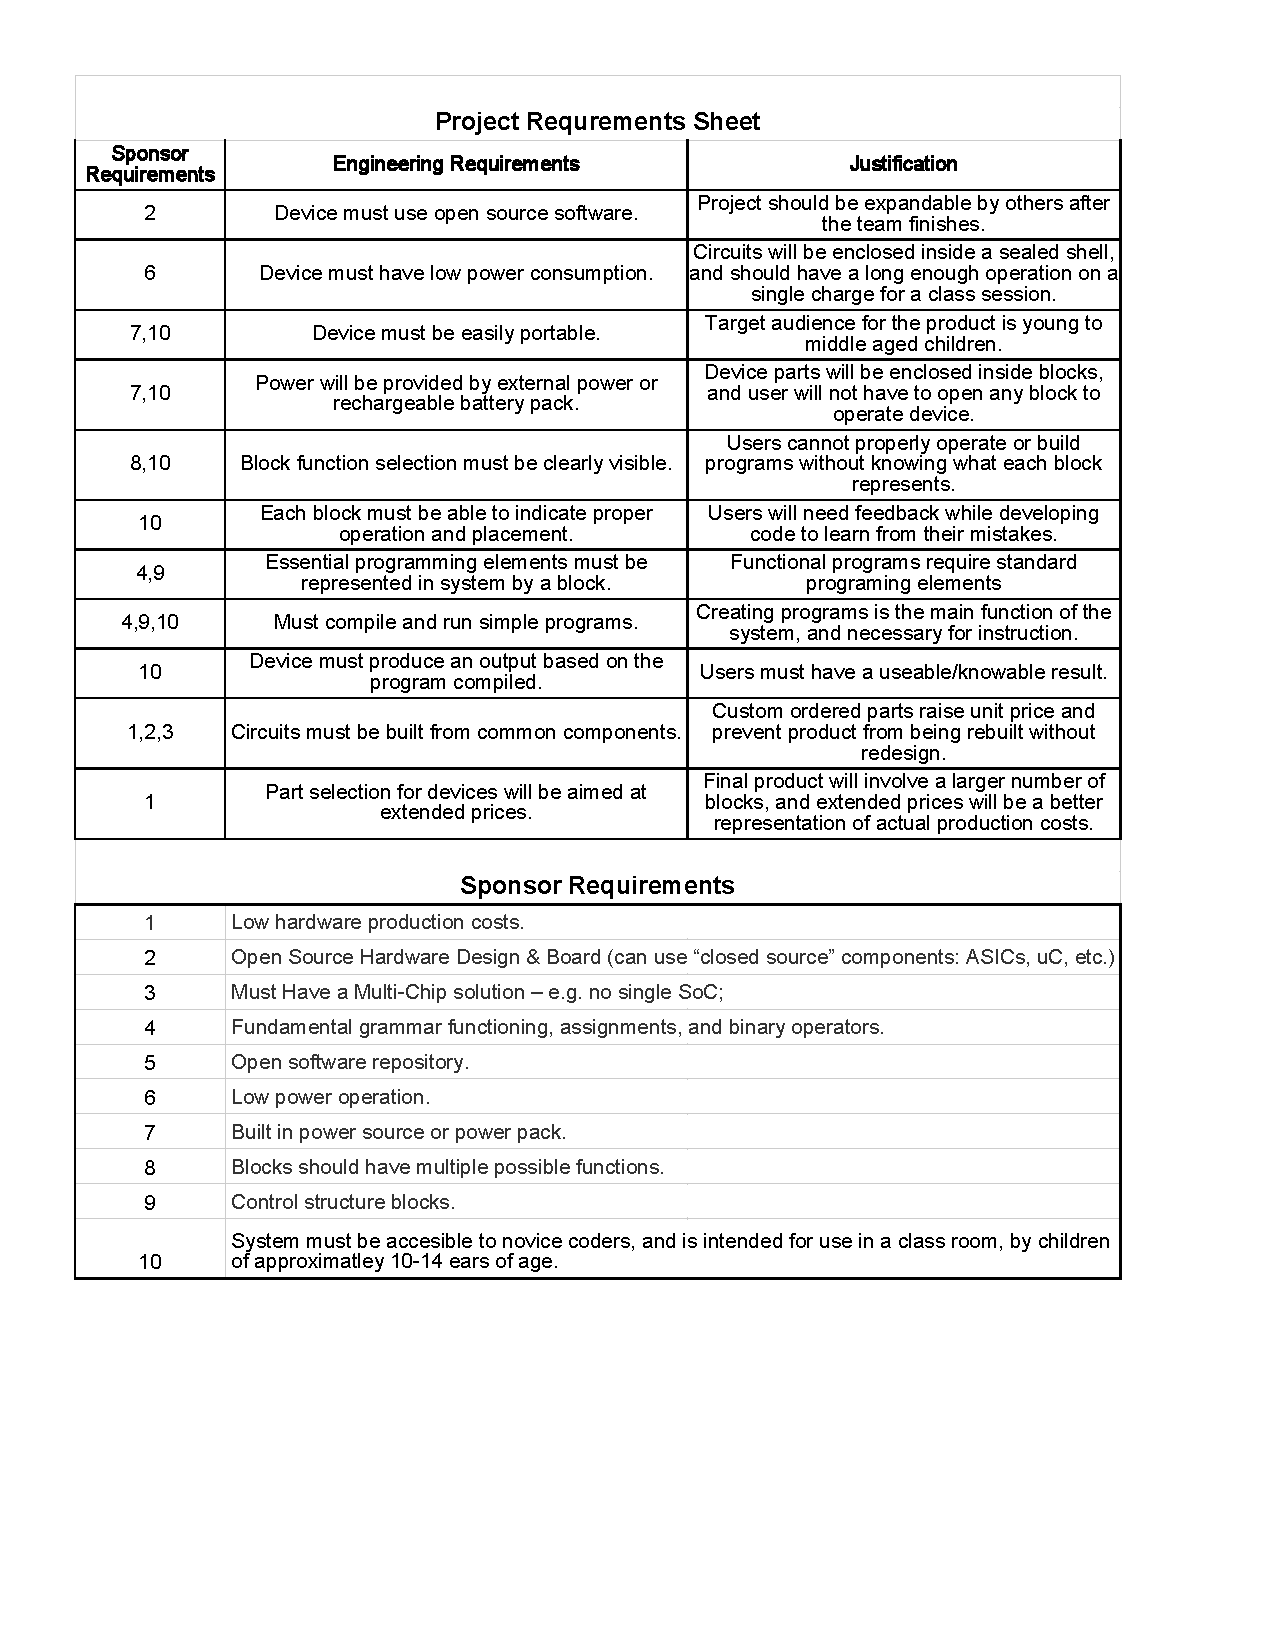
\includepdf[pages={1}]{abcPDS.pdf}
\section{Background}

Currently there are limited methods of teaching  younger groups of students about computer programming, and those that do exist often rely heavily on access to computers. This project is meant to produce a learning aid that will function in a classroom setting, doing away with the need have computers present for learning about programming.
The use of a visual-tactile system to teach new skills to children has a long and well established history dating at least as far back as Froebel, who believed that freedom to play and experiment was essential to real learning.

 In terms of this project the system can be thought of as a, Froebel \textit{Spielgaben}, or a subject specific learning module. The purpose of which is to allow students of any age to be introduced to coding using a familiar process that promotes creativity. Allowing the module to be untethered, separate from a computer, will also allow the teaching of programming without the other distractions available on a PC, and give students that have trouble with abstraction a set of objects to focus on.

\section{Marketing Requirements}


The final package will be a set of between twenty to thirty blocks typically two or less inches across a side. The set will function as it's own interface device, where the topographical arrangement of elements (blocks) will determine the \textit{program}. The individual blocks must be identifiable as belonging to a specific programming construct-group. At a minimum these groups must include; numbers, variables, operators, and controls.

Additionally , if possible, a block should be capable of indicating what  value or function has been  assigned to it. Blocks should be easy to assemble,  allowing users to experiment with layouts, but provide area specific error feedback and thereby increasing understanding and limiting confusion.

Finally, the set should open source and be sufficiently accessible, both by cost and teaching use, as to promote universal access and encourage development and expansion by others.



\section{Risk Management}
Identifying potential risks  at the beginning of a project can help by allowing a certain amount of mitigating action to be built in to the design process.
\subsection{Defining Risks}

 \hspace{.35cm} \textbf{Risk types:}
 \begin{enumerate}
 \item \textbf{Scope}; risks of scope are those that cause the project to be delayed, too complex, or trivial. Frequently these are cause by poorly defined project specifications, attempting to do much, or becoming unnecessarily focused on specific details.
 \item \textbf{Conceptual}; risks belonging here are the products of some failure in understanding a problem or it's intended solution. One example could be  attempting to predict position by triangulation but forgetting to consider velocity.
 \item \textbf{Physical}; risks of this type include problems that manifest physically, most commonly refereed to as \textit{bugs}(software bugs \textit{are} included here. )
 \item \textbf{Incalculable}; risks of this nature include random and unforeseeable events. Shipping delays, inclement weather, and distributor component substitution are all examples of such risks.
 \end{enumerate}
 \subsection{Mitigating Risk}
  \hspace{.35cm} \textbf{Action by type:}
  \begin{enumerate}
  \item \textbf{Scope};
  \begin{enumerate}
  \item Over reaching and scope creep;

  Controlling the scope size can usually be implemented by instituting system of interdepartmental checks, and by setting project goals by stages. The later, infers making the scope such that it satisfies only the minimum project specifications, while the former, in this case infer double checks are done between team and advisor, or other available expert resources.

  In both cases the scope can be added to, but by building a semi-bureaucratic requirement into the process, the chances of adding unrealizable goals to the project have been reduced.
  \item Built in obsolescence;

  In contrast to point (a) is the risk defining the project so precisely as to reduce the final product's usability. Incorporating  mandatory reviews of tasks/ goals at milestones , and use of a check list or pre-scripted questionnaire can help ensure essential functionality has not been overlooked.

  As in the above (5.2 1a) process, by conceiving each stage of the  project between milestones as a singular smaller projects, we improve the chances of including new and relevant additions to scope.
   \end{enumerate}
  \item \textbf{Conceptual};
  \begin{enumerate}
  \item Improperly defined problems;

  The methods of limiting these types of risk are very closely related to those of controlling scope. By ensuring clarity of scope, it then becomes easier to dissect the problem as it pertains to project.

  After dissection, it is up to each team member to voice any concerns or confusions. To which as a group, providing an open, non-judgmental forum is imperative.
  \item Fallacious solution sets;

  This type of risk usually, but not always, stems from having improperly defined problems, which we have  addressed already. For the cases not covered, a solid system of review and collaboration, combined with weekly meetings will reduce the likelihood of implementing improperly framed or proposed-solutions.

  \end{enumerate}
  \item \textbf{Physical};
  \begin{enumerate}
  \item Mechanical;

  Mechanical failure can be difficult to foresee, however by rigorously checking each proposed design for possible simplifications can help mitigate potential pitfalls. General mechanical design considerations should always consider; least number of [connections, moving parts, seams, joints]
  \item Electrical:

  As with mechanical, where checks should also include maximum dissipated power, potential bounces, and bit drift.
  \item Code based;

  Some of the electrical/ mechanical risks can be mitigated with software, however constant review and sections-testing is necessary to ensure that new bugs are not introduced with coded solutions.  Before considering a section done, all attempts should be made to break it.


  \end{enumerate}
  \item \textbf{Incalculable};
  \begin{enumerate}
  \item Components;

  While the very nature of this section precludes prediction, there are certain actions that can limit damage done in event of component based problems. Problems may include, random device failure, shipping delays, distributor substitutions, and more.
  \begin{enumerate}
  \item avoid dependence on non generic components
  \item avoid, where possible, proprietary technologies.
  \item always check licensing
  \item never order minimums
  \item always build in parallel
  \end{enumerate}
  \item Events;

  The most effective way to mitigate damages done by events like unforeseen weather or closure of services needed, is to have a flexible, organic schedule (see next).
  \item Scheduling;

  Designing a system of scheduling, that allows for the most efficient use of available resources can greatly reduce strain on project time-lines. For this project we have implemented a generic, \textit{by ticket} system, which allows team members to \textit{bid} on project tasks as dictated by their own constraints. This combined with ensuring that no individual task is longer than the time between meetings (1-week) will help ensure work flow.
  \end{enumerate}
  \end{enumerate}

\section{Current Proposed Solutions }
  The current solutions we propose below are subject to change, as feasibility and effectiveness will become more clear as prototyping commences. Each level of description is limited to an overview in this paper, as we address each solution further in the \textit{Product  Specifications} document. The overviews are given to give enough familiarity to address the \textit{pitfalls} subsection.

\subsection{System Overview and User Interface}
 Our product will consist of identical \textit{blocks}, each with enough digital circuitry to accomplish the next subsection. Blocks will electrically connect with one another via metal-on-metal contact, forming a grid. Some of these metal nets will form a mesh grid (local communication), while some of them will form a global bus (power and I2C-or-similar bus). We will address this network as a \textit{matrix} in this paper.

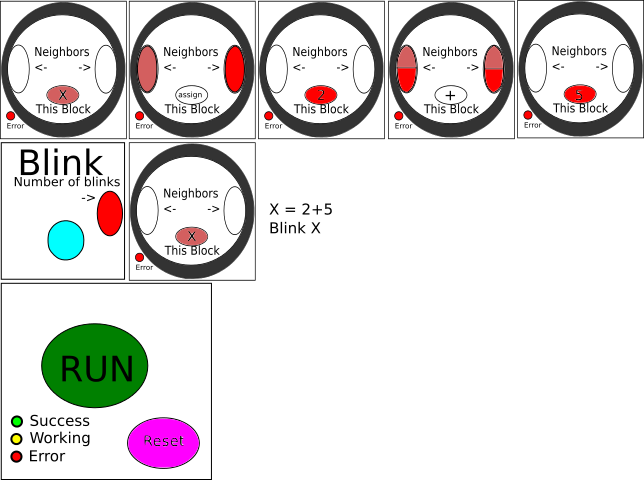
\includegraphics[width=6in]{user_interface}
\vspace{.5cm}\\
The  start block, or control block (see figure), has buttons to  force a reset or to attempt a run/ compile.  It also has LED indicators for relaying current status. It connects to the bottom most left most of the other blocks. \begin{verbatim}
<Note: the bottom is one possible configuration being considered> 
\end{verbatim}

Each programming block connects to its neighbors to form a program. The lines of  code are read from left to right, and lines are read one at a time from top to bottom. On each programming block a tunable wheel allows the user to select the meaning or \textit{value} of the block  in it's \textbf{\textit{This Block}} window.  Users are given hints for which blocks ought to be placed to the left and right of the current block. Hints appear in the \textbf{\textit{Neighbors}} windows, and an LED will indicate error when the program is run if the block sequence is invalid . 

Output blocks will have some way of acting on the world, such as a controllable light source, or a small speaker for sound. The interface to control  output is a separately connected to a special \textit{output} block (not shown), which may be connected to the run/ control block.


   
    On the last line of the matrix, Row 1, the user will place the Master Processing block, which is not identical to the other blocks.
  \subsection{Blocks And Communication: Software}
    Each block stores its own associated data. Each block stores a \textit{position vector}, which represents where on the matrix the block is located, and stores a \textit{unique ID}, which allows the block to be uniquely addressed on the global bus. Upon initialization, the position vector of each block is unknown.
   
    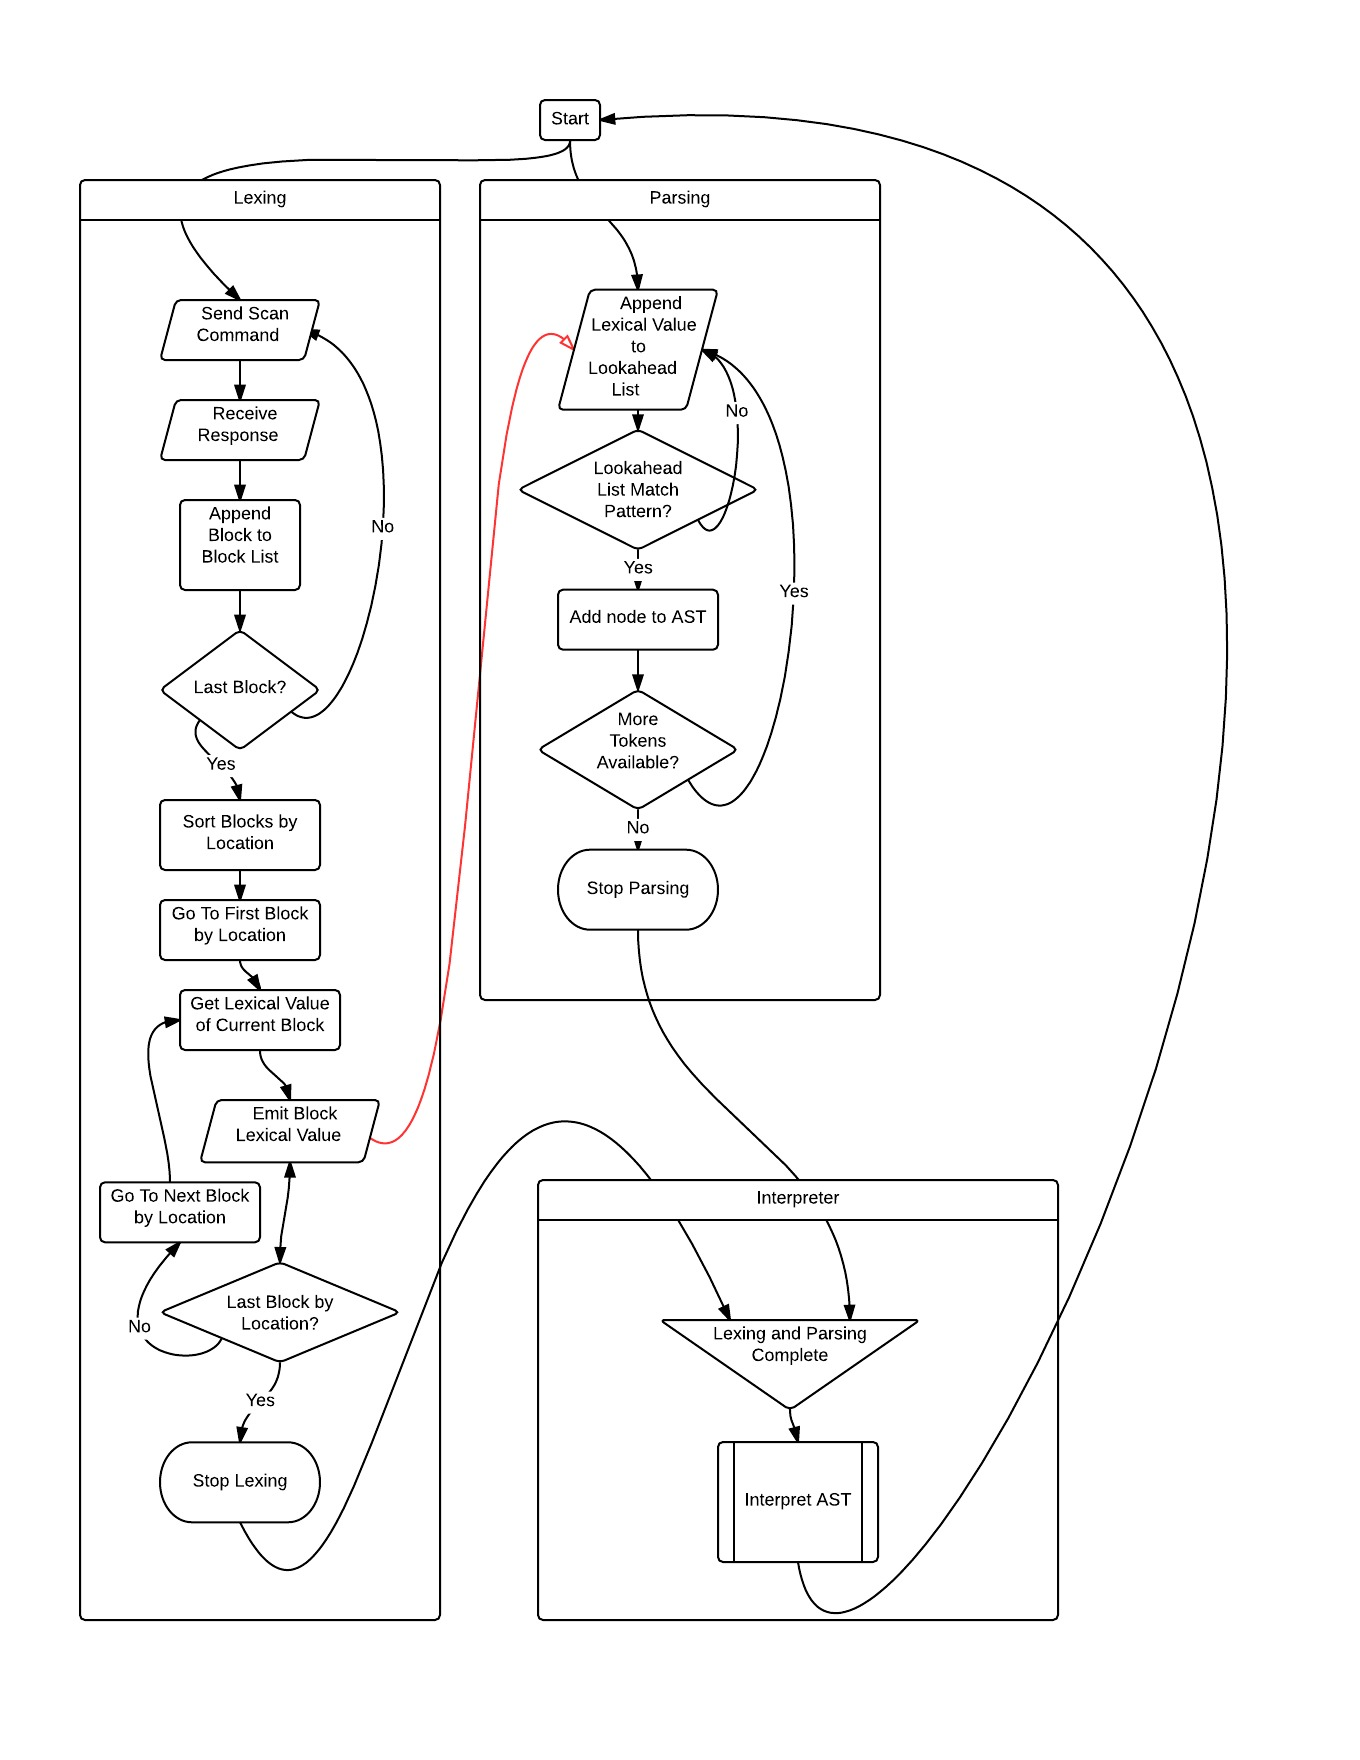
\includegraphics[width=6in]{central_processor_stages}

    \subsubsection{Determining Location}
      The process for each block to identify its position vector is as follows:
      \begin{enumerate}
        \item First the positions of each block in column 1 are discovered:
        \begin{enumerate}
          \item The processing block passes a \begin{verbatim}<0,0>\end{verbatim} vector to its northern neighbor via the local bus.
          \item Until the end of the column is reached, whenever a block receives a vector from its southern neighbor, each block increments the y component of its position vector, emits a message on the global bus containing \begin{verbatim}[position vector, unique ID]\end{verbatim}then passes its position vector to its northern neighbor.
          \item The last block on the column increments the y component of its position vector, then emits a message on the global bus containing \begin{verbatim}[position vector, unique ID, END_OF_DIMENSION]\end{verbatim}
        \end{enumerate}
      \item The processing block collects this info in its own local-cache of the matrix.
      \item To identify each block in each row:
        \begin{enumerate}
          \item The processing block iterates over each Column 1 entry in its local-cache. Using the emitted Unique IDs for each entry, the processing block sends a \begin{verbatim}BEGIN_RASTER\end{verbatim}message to each Column 1 block via the global bus.
          \item When each Column 1 block receives a \begin{verbatim}BEGIN_RASTER\end{verbatim}message on the global bus, it passes its Position Vector to its eastern neighbor via the local bus.
          \item Until the end of the line is reached, whenever a block receives a vector from its western neighbor, each block increments the x component of its position vector, emits a message on the global bus containing \begin{verbatim}[position vector, unique ID]\end{verbatim}then passes its position vector to its eastern neighbor.
          \item The last block on the line increments the x component of its position vector, then emits a message on the global bus containing \begin{verbatim}[position vector, unique ID, END_OF_DIMENSION]\end{verbatim}
        \end{enumerate}
      \item Using the messages passed on the global bus, the processing block is able to fill in its local-cache with all of the Unique IDs of the blocks in the network.
      \end{enumerate}
  \subsection{Language, Parsing, Processing}
    After filling in its local-cache, the processing block can interpret the language in a traditional manner using a Lexer, Parser, and AST-Interpreter. This all happens in software.
    \subsubsection{Lexing}
      The processor is coded with an alterable lookup table containing the token associated with each Unique ID. The lexer does a raster scan on the processors local-cache matrix, and for each Unique ID it encounters, looks up the lexical value of the ID in the lookup table. The lexer hands this token to the Parser.
    \subsubsection{Parsing}
      The parser is a traditional LR parser that constructs an abstract syntax tree from the lexical tokens handed to it by the lexer. It passes the root of the abstract syntax tree to the interpreter.
    \subsubsection{Interpretation}
      The interpreter descends the abstract syntax tree, performing the actions associated with each node.\\
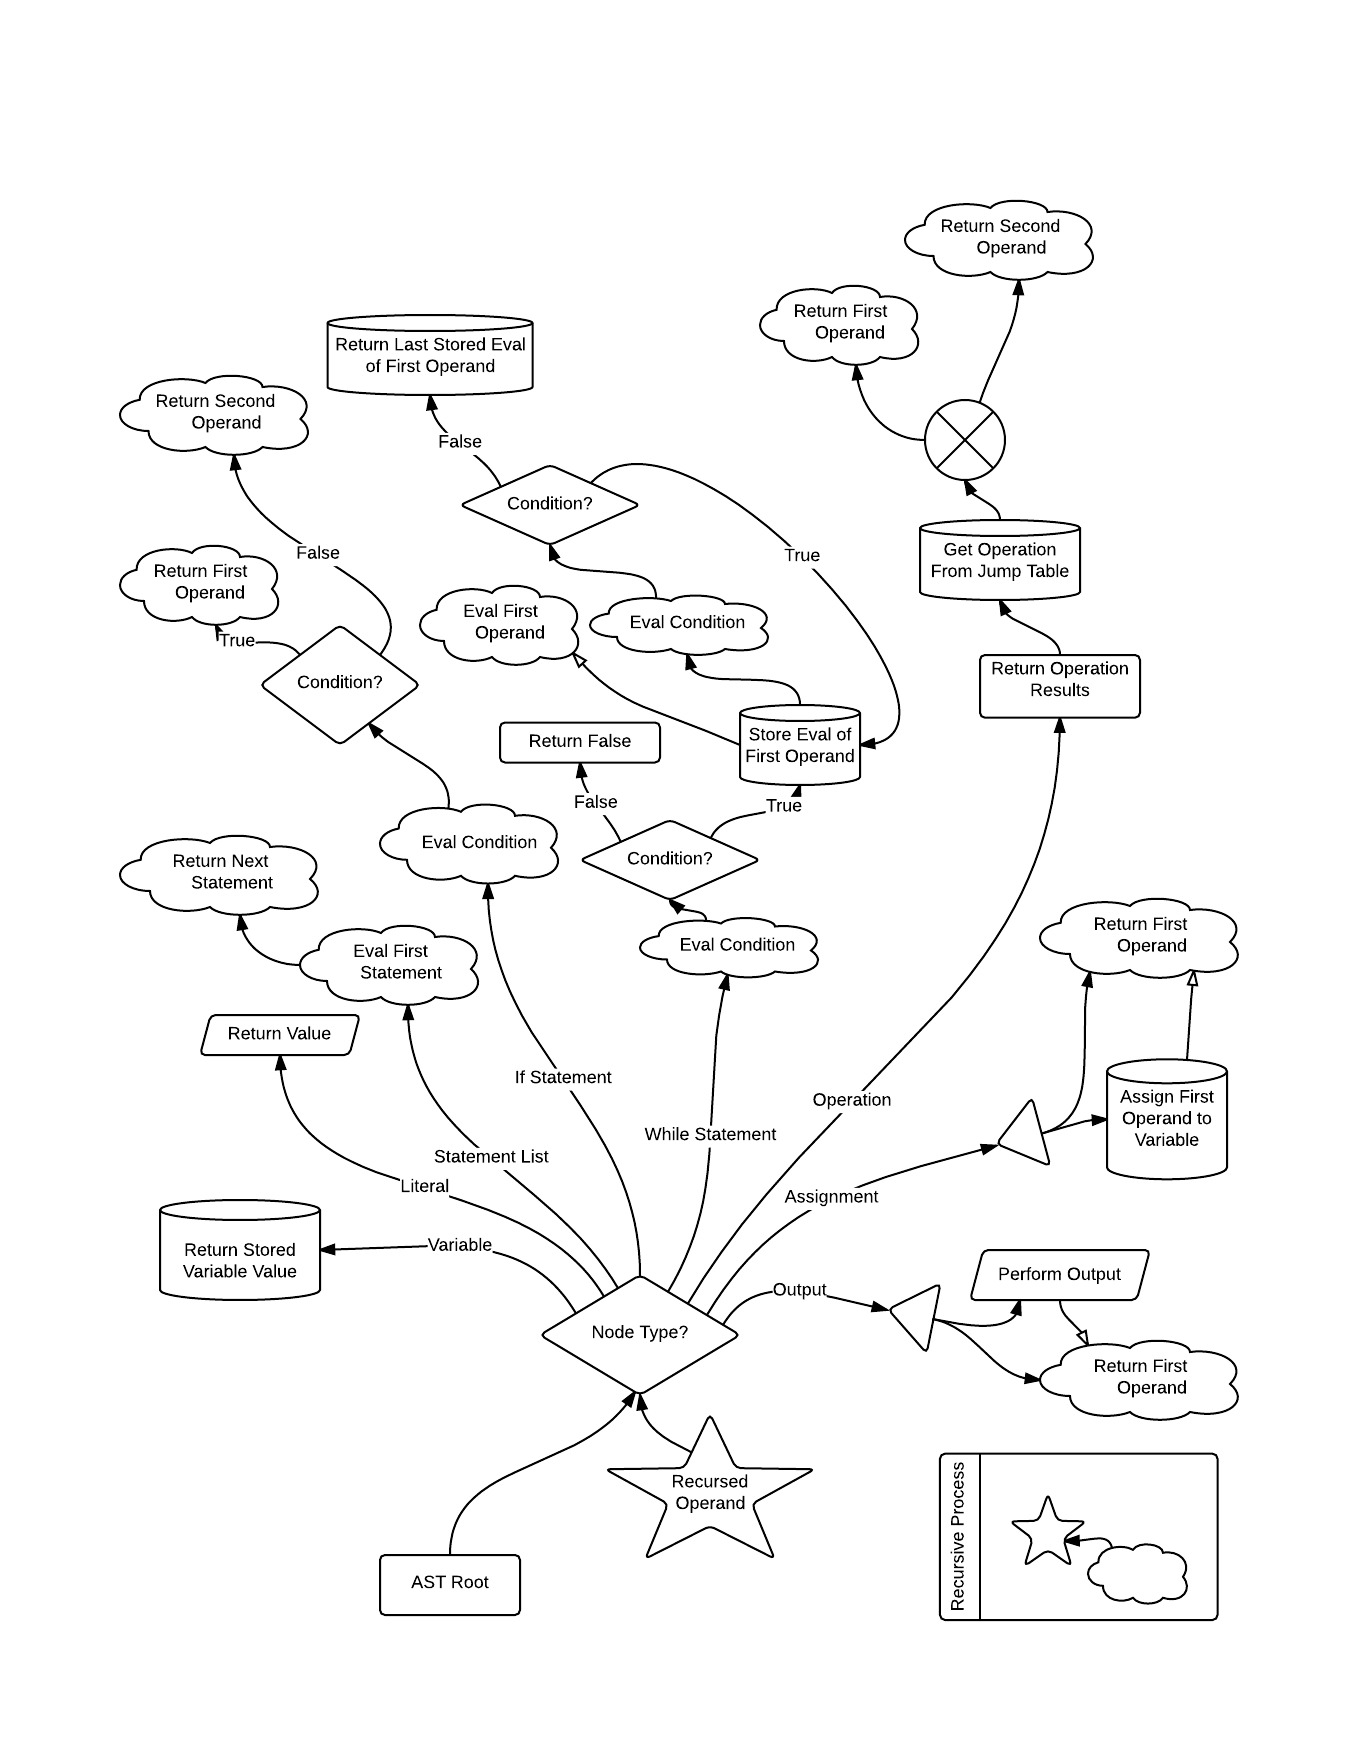
\includegraphics[width=5.5in]{central_processor_interpreter}
\subsection{ Visual Feedback}
Currently the scheme for allowing the user to set the  block token (see 6.3.1) to be handed to the parser involves a system of selectable visual cues on the top face of the block. Either a rotary encoder or potentiometer will be attached to a coded wheel that sits under the top face of the block, with a radius such that just the edge of the wheel maybe manipulated by the user through a cut out on the side face of the block (see figures below).
\subsubsection{Wheel Encoder Diagrams}
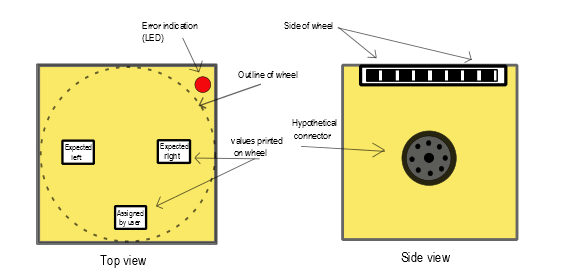
\includegraphics{BlkFace.png}
\subsubsection{I/O}
User interface by rotating the wheel to select the desired value (token), this corresponds to a number processed via Grey Code or ADC which is then sent to the lexer for lookup.

When the interpreter has finished compiling the program image, if any errors exist, the control unit identifies which unique ID holds the token that caused it and sends out on the bus;
\begin{verbatim}
[unique ID]
FLASH_LED
\end{verbatim}

\subsection{Micro-controller}

\includegraphics[width=6in]{uC_State}
Once a micro-controller has determined its address, it will enable its I2C port and attach itself to the shared bus. This allows the main processor SBC to regularly poll the bus for the correct devices.
\begin{verbatim}
<Note: I2C is one possible protocol being considered>
\end{verbatim}
The diagram on the previous page assumes that the main processor \textbf{block} is oriented at the bottom-left of the code blocks and the \textbf{program} will be built up from this origin, i.e. each block receives its position vector either from below or from the left. 


This implementation allows us to utilize existing, supported, documented I2C drivers for both the micro controller in a hardware-supported and interrupt-driven slave-mode and the SBC in master-mode.

If the block is disconnected and reconnected it should return to the beginning state. This is now noted at the top by Reset.

In a 2x2 example, the block at (1, 1) would get vector signals both from the left and from below. It could simply use the first one it receives and ignore the other, or it could use the second to confirm the correct position as they should generate the same coordinate value.


Each micro-controller generates its own address from its position vector. A possible implementation is that the x-coordinate is the most significant 3 bits of the address, followed by the y-coordinate as the next 4 bits of the address, and the final bit (LSB) is the I2C R/W bit, per spec. For example, the block at position (2, 1) would have the address of: [010 0001 x]. This resolves to dimension limitations of 8 blocks long and 16 blocks tall, or a max 16 lines of code that are max 8 blocks wide. This is further limited by I2C reserved addresses. Other implementations could improve upon this.


Once the block knows its function and its position, it is immediately available for I2C addressing from the SBC. Since the I2C communication will be interrupt-driven, the block can resume setting up after it services a message if it was received before it completed initialization. Possible commands could include:
\begin{verbatim}
* Return this block's function code
* Toggle this block's error LED
* Reset this block
* Etc.
\end{verbatim}
   
\subsection{Physical Connections}
Blocks will be interlocked using small outward pegs with corresponding recessed cavities. These protrusions on the blocks will contain the electrical connectors, and serve as a physical guide to ensure the pin connections line up during product use. A combination of varying the connector types, the protrusion shapes, and magnets can be used to hold blocks firmly together and  will ensure that only the correct face of one block can be mated to a second block.\\
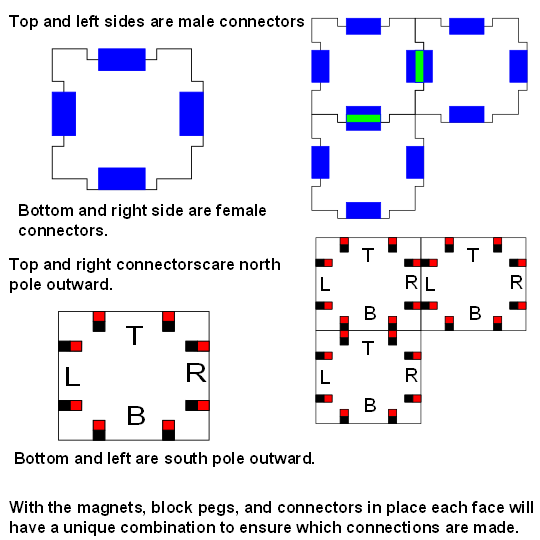
\includegraphics[width=5in]{Connector_scheme_Drawing}


  \section{Pitfalls}
  \subsection{User Interface}
  In any scheme designed to be easy to use there is the danger of being easy only for the designers. What we think of as intuitive is not certain to be easy to understand for students or teachers. 
  The more complex our manuals or instructions are, the clearer it can be how to use the blocks. However there is a limit to how much time a  user is willing invest in reading instruction before they can use the blocks effectively . If there is not enough or too much user targeted documentation, learning to use the blocks could be frustrating.
  The solution to both of those dangers appears to be testing, which invites a trade off of time and resources spent on testing versus spent on designs and implementations. 
  \subsection{Software}
    Possible pitfalls for the current proposed solution are discussed in this section, and likely mitigation techniques are discussed for each pitfall.
    \begin{enumerate}

      \item Varying path lengths on each bus may result in bit drift and/or clock skew.
      \begin{enumerate}
        \item \textit{Mitigation:} Throughput on buses is not likely to be a significant factor in system performance (whereas interpreter performance is), so slower baud rates are a cheap solution.
      \end{enumerate}

%   WE DO NOT CURRENTLY ADDRESS 2 DIMENSIONAL SCANNING IN OUR PAPER, WE ONLY INTRODUCE RASTER SCANNING TECHNIQUE
%      \item Propagation of position vectoring commands along two dimensions could result in long wait times for global bus arbitration, resulting in timeouts.
%      \begin{enumerate}
%        \item
%      \end{enumerate}

      \item A user can write an infinite loop
      \begin{enumerate}
        \item \textit{Mitigation:}User programs will run in their own process which will be killed whenever blocks are rearranged (then the new program will start in a new process).
      \end{enumerate}

      \item Manufacturing uncertainties: Connectors do not align; enclosures are not square. Magnetic interference.
      \begin{enumerate}
        \item \textit{Mitigation:} Expose connectors for proof-of-concept revisions to demonstrate functionality.
      \end{enumerate}

      \item Communication algorithm was inherently flawed.
      \begin{enumerate}
        \item \textit{Mitigation:} We plan to release our first revision at the halfway mark before "product launch". Reimplementing the Location-Vectoring algorithm using a tray as a fixed-grid reader of Unique IDs would be trivial from a design perspective.
      \end{enumerate}

    \end{enumerate}
   
   \subsection{Visual Feedback}
   In general there is a proportional relationship between the level of detail relayed to the user and complexity. The current proposal involves several moving pieces which each represent a risk of mechanical failure. Additionally there is a hardware to software interface at each point that posses additional risks. 
   
   By contrast limiting the feedback system runs the risk of making the program controls too difficult.  Use of an ID stub in software will help mitigate the HW/ SW interface risks and we will remain willing to limit the number of selectable states if need be. In this first run  we may also have to use a simple dial without the encoded wheel as proof of concept.
   \subsection{Micro-controller}
   
   Blocks may get stuck in different states. Reset triggers and watchdog timers can help alleviate some issues. Additionally the algorithm on its own does not determine end of line or completed search, the main processor block must poll regularly for block identities. This can lead to:
      \begin{verbatim}
       * Stale function values
       * Wasted processing on both ends of the bus
      \end{verbatim}
     
   Possible optimizations can be made by limiting poll to likely addresses (blocks starting at 0, etc)
    \subsection{Physical Connections}
    The interlocking of the blocks adds the possibility that blocks can only be inserted easily on faces that have no adjacent blocks already connected. This would mean that if the interlocking sections of blocks are tight tolerance, rows will have to be constructed prior to being connected to other rows. How close of a tolerance is required will also determine what kind of mounting is use for the connection. If the blocks will tightly interlock then a panel mount connect can be used to prevent mechanical stress from reaching the circuit board. If a more flexible or loose fitting interlock is found to be required then attaching the connectors to the block walls isn't an option, and a firm but flexible mounting option will be required.
    
    Adding a magnetic connection to hold the blocks together makes assembly of the block more difficult. Having unique locations for each connector/interlock pair means that an incorrectly oriented magnetic internal to the device could prevent a good connection.
    

\end{document}{
